%%%%%%%%%%%%%%%%%%%%%%%%%%%%%%%%%%%%%%%%%%%%%%%%%%%%%%%%%%%%%%%%%%%%%%
% Problem statement
\begin{statement}[
  problempoints=110,
  timelimit=1 second,
  memorylimit=512 MiB,
]{Džumbus}

\setlength\intextsep{-0.1cm}
\begin{wrapfigure}[7]{r}{0.23\textwidth}
\centering
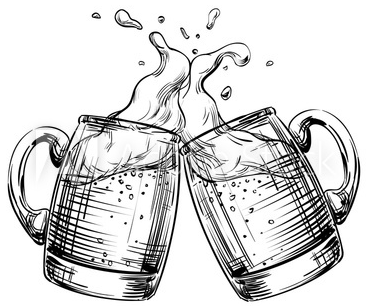
\includegraphics[width=0.23\textwidth]{img/dzumbus.png}
\end{wrapfigure}

%\subsection

Marin is a good man, so he'll organize $Q$ parties for his $N$ friends, all of
which are competitive programmers. The only drink that is going to be served at
his parties will be \textit{džumbus} --- a mixture of Coke and ginger juice.

For each of his friends, Marin knows the amount of džumbus they need to
drink in order to relax. He also knows that there are $M$ pairs of people among
his friends such that, if both of them are relaxed, they will begin to
exchange the solutions of past COCI problems (since there are no
published editorials). When a person $A$ shares their solutions with person $B$,
the person $B$ may decide to share those solutions in the same manner, but it is
also known that $M$ pairs are formed in a way that it is impossible that those
solutions will get back to person $A$ during that party, regardless of the order in
which exchanges took place.

Marin has prepared different amounts of džumbus for each party. During each
party, he will distribute the drink in a way which maximizes the number of
people that will at least once exchange their solutions with another person
at that party.

Your task is to determine the number of people that will exchange their
solutions for each of the $Q$ parties.
%%%%%%%%%%%%%%%%%%%%%%%%%%%%%%%%%%%%%%%%%%%%%%%%%%%%%%%%%%%%%%%%%%%%%%
% Input
\subsection*{Input}
The first line contains integers $N$ and $M$ from the task description. \\
The second line contains $N$ space separated integers $D_i$, the amounts of
džumbus needed to relax Marin's friends, given in order from a friend number $1$
to a friend number $N$. \\
The $i$-th of the next $M$ lines contains two integers $A_i$ and $B_i$
$(A_i \ne B_i)$, denoting a pair of friends from the task description. \\
The next line contains an integer $Q$ from the task description. \\
The next $Q$ lines contain a single integer $S_i$ which represents the total
amount of džumbus that is going to be served at $i$-th party.


%%%%%%%%%%%%%%%%%%%%%%%%%%%%%%%%%%%%%%%%%%%%%%%%%%%%%%%%%%%%%%%%%%%%%%
% Output
\subsection*{Output}
Output the number of people that will exchange their solutions for each
of the $Q$ parties. The answer for each party should be given in a separate
line. Note that the parties are independent of each other.

%%%%%%%%%%%%%%%%%%%%%%%%%%%%%%%%%%%%%%%%%%%%%%%%%%%%%%%%%%%%%%%%%%%%%%
% Scoring

\subsection*{Scoring}
In all subtasks, it holds $0 \le M < N \le 1000$, $1 \le Q \le 2\cdot10^5$,
$1 \le D_i \le 10^9$ and $1 \le S_i \le 10^9$.

{\renewcommand{\arraystretch}{1.4}
  \setlength{\tabcolsep}{6pt}
  \begin{tabular}{ccl}
 Subtask & Score & Constraints \\ \midrule
  1 & 20 & \makecell[l]{$M = N - 1$, $1 \le S_i \le 1000$, \\
            Marin's friends will be paired up in a way that each friend \\
            will exchange their solutions with at most two other people.} \\
  2 & 30 & \makecell[l]{$M = N - 1$ \\
            Marin's friends will be paired up in a way that each friend \\
            will exchange their solutions with at most two other people.} \\
  3 & 30 & $N \le 100$ \\
  4 & 30 & No additional constraints. \\
\end{tabular}}

%%%%%%%%%%%%%%%%%%%%%%%%%%%%%%%%%%%%%%%%%%%%%%%%%%%%%%%%%%%%%%%%%%%%%%
% Examples
\subsection*{Examples}
\begin{tabularx}{\textwidth}{X'X'X}
\sampleinputs{test/dzumbus.dummy.in.1}{test/dzumbus.dummy.out.1} &
\sampleinputs{test/dzumbus.dummy.in.2}{test/dzumbus.dummy.out.2} &
\sampleinputs{test/dzumbus.dummy.in.3}{test/dzumbus.dummy.out.3}
\end{tabularx}

\textbf{Clarification of the third example:}
At the first party, Marin decided to relax friends with indexes
$1$, $2$, $3$, $7$, $9$, $10$, $12$ and $13$. They have drunk a total
of $45$ units of džumbus.

\setlength\intextsep{-0.5cm}
\begin{wrapfigure}{c}{\textwidth}
\centering
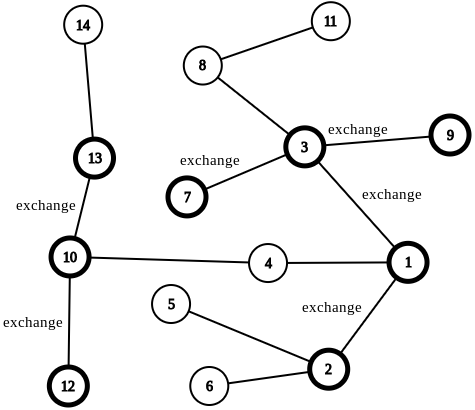
\includegraphics[width=0.6\textwidth]{img/treeEnglish.png}
\end{wrapfigure}

%%%%%%%%%%%%%%%%%%%%%%%%%%%%%%%%%%%%%%%%%%%%%%%%%%%%%%%%%%%%%%%%%%%%%%
% We're done
\end{statement}

%%% Local Variables:
%%% mode: latex
%%% mode: flyspell
%%% ispell-local-dictionary: "croatian"
%%% TeX-master: "../hio.tex"
%%% End:
